\documentclass[tikz,border=2mm]{standalone}
\usepackage{pedramsyms}
\usepackage{tikz}
\usetikzlibrary{shapes,arrows,positioning,fit,calc}
\usepackage{amsmath}
\usepackage{amssymb}

\definecolor{green1}{HTML}{E2F0D9}
\definecolor{blue1}{HTML}{DAE3F3}
\definecolor{red1}{HTML}{FBE5D6}

\begin{document}

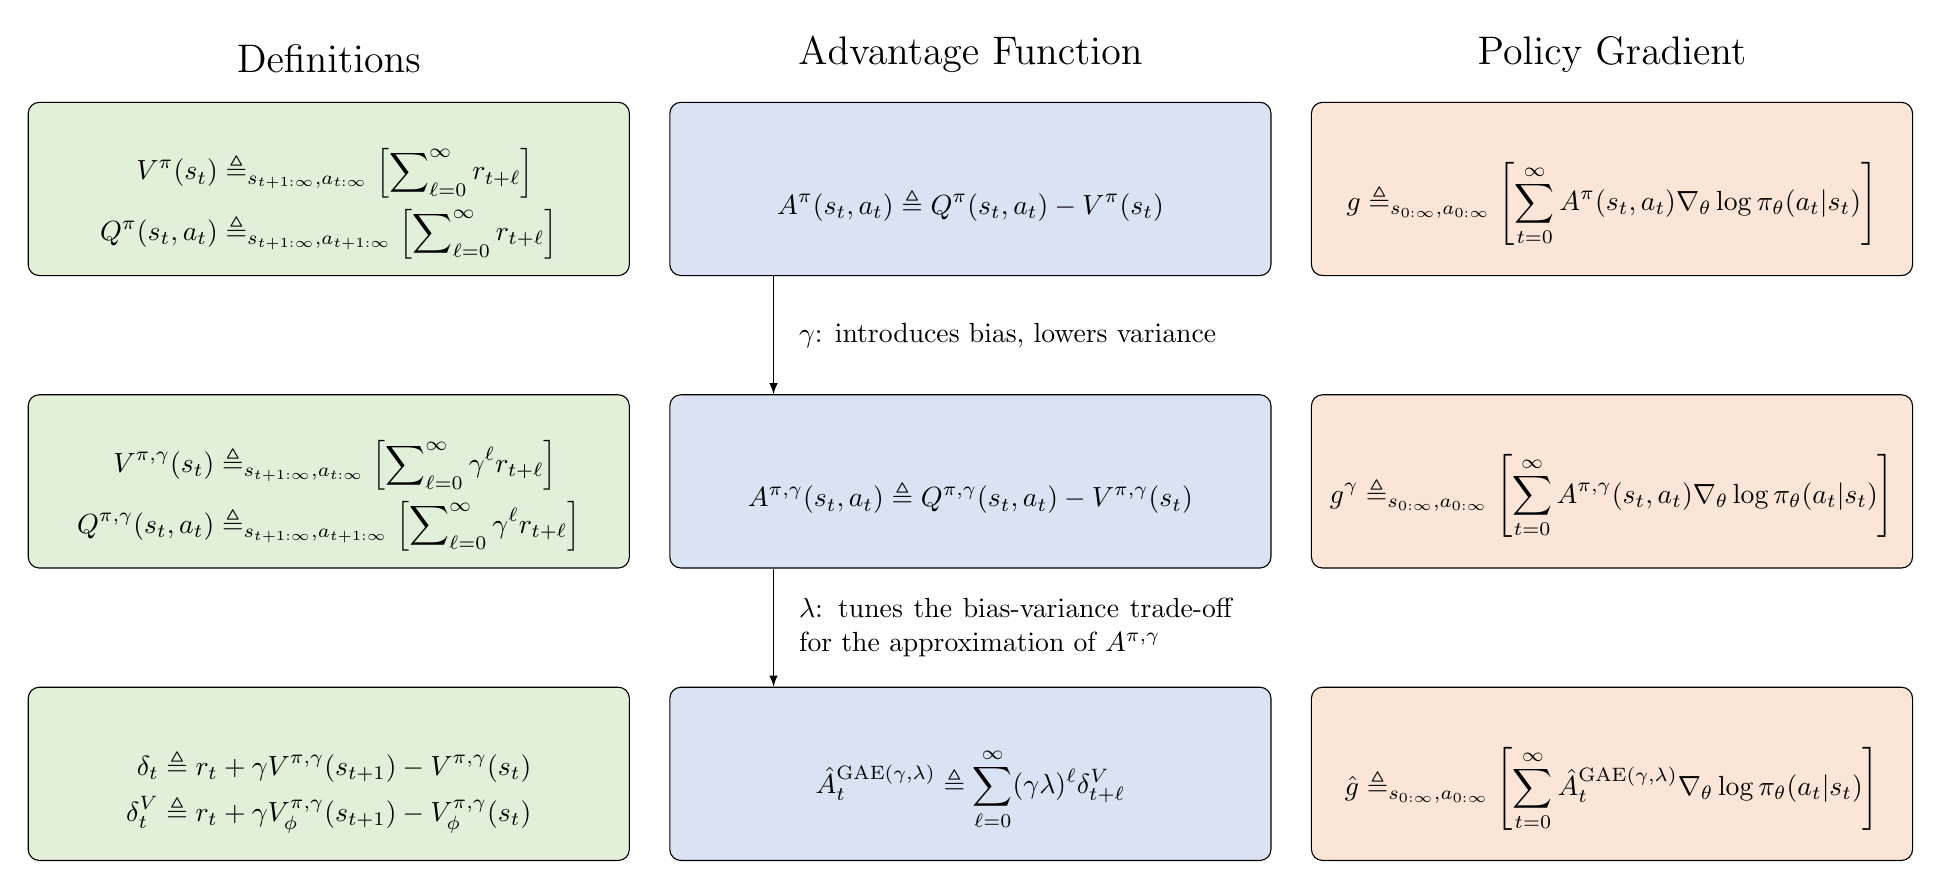
\begin{tikzpicture}[>=latex]

% Define block styles
\tikzstyle{block} = [rectangle, rounded corners, draw, minimum width=7.4cm, minimum height=2.2cm, text centered, text width=7.4cm]

% Nodes
\node (d1) [block,fill=green1] {
\begin{align*}
    V^\pi(s_t) &\triangleq\BBE_{s_{t+1:\infty},a_{t:\infty}}\left[ \sum\nolimits_{\ell=0}^\infty r_{t+\ell}\right]\\
    Q^\pi(s_t, a_t) &\triangleq\BBE_{s_{t+1:\infty},a_{t+1:\infty}}\left[ \sum\nolimits_{\ell=0}^\infty r_{t+\ell}\right]
\end{align*}
};

\node (d2) [block, below=1.5cm of d1,fill=green1] {
\begin{align*}
    V^{\pi,\gamma}(s_t) &\triangleq\BBE_{s_{t+1:\infty},a_{t:\infty}}\left[ \sum\nolimits_{\ell=0}^\infty \gamma^\ell r_{t+\ell}\right]\\
    Q^{\pi,\gamma}(s_t, a_t) &\triangleq\BBE_{s_{t+1:\infty},a_{t+1:\infty}}\left[ \sum\nolimits_{\ell=0}^\infty \gamma^\ell r_{t+\ell}\right]
\end{align*}
};

\node (d3) [block, below=1.5cm of d2,fill=green1] {
\begin{align*}
    \delta_t \triangleq r_t + \gamma V^{\pi, \gamma}(s_{t+1}) - V^{\pi,\gamma}(s_t)\\
    \delta_t^V \triangleq r_t + \gamma V_\phi^{\pi, \gamma}(s_{t+1}) - V_\phi^{\pi,\gamma}(s_t)
\end{align*}
};


\node (a1) [block, right=0.5cm of d1, fill=blue1] {
\begin{align*}
A^{\pi}(s_t,a_t) &\triangleq Q^\pi(s_t, a_t) - V^\pi(s_t)
\end{align*}
};

\node (a2) [block, below=1.5cm of a1, fill=blue1] {
\begin{align*}
A^{\pi,\gamma}(s_t,a_t) &\triangleq Q^{\pi,\gamma}(s_t, a_t) - V^{\pi,\gamma}(s_t)
\end{align*}
};

\node (a3) [block, below=1.5cm of a2, fill=blue1] {
\begin{align*}
    \hat A_t^{\rm{GAE}(\gamma, \lambda)} \triangleq \sum_{\ell =0}^\infty (\gamma\lambda)^\ell \delta_{t+\ell}^V
\end{align*}

};

\node (p1) [block, right=0.5cm of a1, fill=red1] {
\begin{align*}
    g \triangleq \BBE_{s_{0:\infty}, a_{0:\infty}}\left[\sum_{t=0}^\infty A^\pi(s_t,a_t)\nabla_\theta \log \pi_\theta(a_t \vert s_t)\right]
\end{align*}
};

\node (p2) [block,below=1.5cm of p1,fill=red1] {
\begin{align*}
    g^\gamma \triangleq \BBE_{s_{0:\infty}, a_{0:\infty}}\left[\sum_{t=0}^\infty A^{\pi,\gamma}(s_t,a_t)\nabla_\theta \log \pi_\theta(a_t \vert s_t)\right]
\end{align*}

};

\node (p3) [block,below=1.5cm of p2,fill=red1] {
\begin{align*}
    \hat g \triangleq \BBE_{s_{0:\infty}, a_{0:\infty}}\left[\sum_{t=0}^\infty \hat A_t^{\rm{GAE}(\gamma, \lambda)}\nabla_\theta \log \pi_\theta(a_t \vert s_t)\right]
\end{align*}
};

% Labels
\node [above=0.25cm of d1,font=\Large] {Definitions};
\node [above=0.25cm of a1,font=\Large] {Advantage Function};
\node [above=0.25cm of p1,font=\Large] {Policy Gradient};

\draw [->] ([xshift=-2.5cm]a1.south) -- node[pos=0.5,right,xshift=0.2cm] {$\gamma$: introduces bias, lowers variance} ([xshift=-2.5cm]a2.north);

\draw [->] ([xshift=-2.5cm]a2.south) -- node[pos=0.5,right,xshift=0.2cm]  {\parbox[c]{5.5cm}{$\lambda$: tunes the bias-variance trade-off for the approximation of $A^{\pi, \gamma}$}}  ([xshift=-2.5cm]a3.north);

\end{tikzpicture}

\end{document}